% !TEX root = ../../main.tex

\section{Consistency models}

\section{Data structures}

\section*{State of the art Key Value Store}

\section{Consistency issues}

% let me remind the rules at Sorbonne Univ.
% (french version below).

% \section{The detailed steps of the defence}
% \label{sec:ec:detailed-steps-of-the-defencev}

% \begin{figure*}[tp]
%     \centering
%     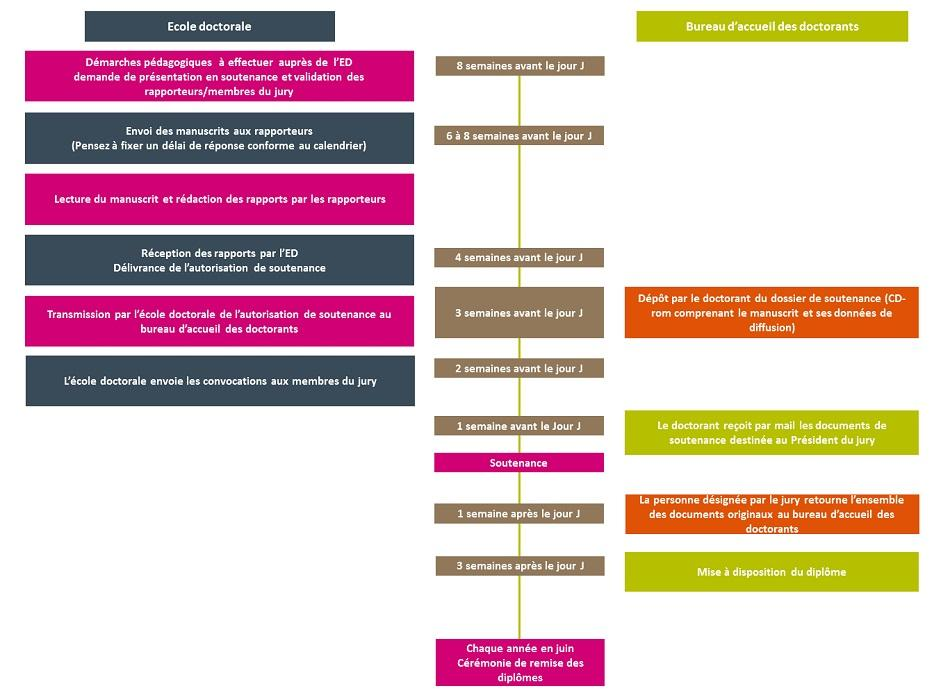
\includegraphics[scale=0.7]{figures/etapes_soutenance.jpg}
%     \caption{Admin steps of the defence.}
%     \label{fig:etapes-soutenance}
% \end{figure*}

% \section{The manuscript}
% \label{ch:the-manuscript}

% \paragraph{Language of the manuscript}

% As the thesis leads to the award of a French national degree, it should generally be written and defended in French. However, it may be the case that, for scientific reasons, the subject matter requires the use of a language other than French. By decision of the Scientific Council of 4 March 2013, this is now decided by the directors of doctoral schools, who are competent to judge matters of scientific priority.
% As recommended by the Ministry, a lengthy written summary of the thesis in French will be required.

% \paragraph{Writing the manuscript}

% To help you write your manuscript, Sorbonne University provides you with a guide for writing and presenting theses, as well as two style sheets, one of which concerns international co-supervision theses.

% \begin{itemize}
%     \item Guide to writing and presenting theses
%     \item Classic style sheet
%     \item \emph{Style sheets:} theses in international co-supervision
% \end{itemize}

% Communication courses are organised for the preparation of your manuscript but also for the defence. Find these courses in the training catalogue for doctoral candidates at Sorbonne University. 

% \section{Appointment of rapporteurs and the thesis jury}
% \label{sec:appointment-of-rapporteurs}

% The President of Sorbonne University delegates the appointment of rapporteurs, the composition of the jury and the authorisation of the defence to the director of the doctoral school.

% \paragraph{Appointment of rapporteurs}

% The President appoints two rapporteurs, authorised to direct research or belonging to one of the categories referred to in Article 17 of the Order of 25 May 2016 at the proposal of the director of the doctoral school and after consulting the thesis director.

% \begin{itemize}
%     \item Rapporteurs must come from outside the doctoral school and the doctoral candidate's institution of enrolment.
%     \item They have no involvement in the work of the doctoral candidate.
%     \item They may come from foreign higher education or research institutions or other foreign bodies.
%     \item The rapporteurs shall make their opinion known by means of written reports on the basis of which the President shall authorise the defence. These reports shall be made known to the jury and the candidate before the defence.
%     \item In the event of disagreement between the two rapporteurs, the President shall appoint a third rapporteur.
% \end{itemize}

% \paragraph{Appointment of the thesis jury}

% The thesis jury is appointed by the president after consulting the director of the doctoral school and the thesis director.
% There are between 4 and 8 jury members.

% At least half of its members are French or foreign people, from outside the doctoral school and the candidate's enrolment establishment, chosen for their scientific competence, subject to provisions relating to the international co-supervision of the thesis. At least half of the jury must be made up of professors or similar personnel, or teachers of equivalent rank who do not report to the Ministry in charge of higher education. Its composition must allow a balanced representation of women and men. The thesis director is a member of the jury, but does not take part in the decision.
% The thesis jury must include, apart from the thesis director, a lecturer or researcher from Sorbonne University - i.e. attached to a research structure associated with Sorbonne University - holding accreditation to direct research or similar.

% \section{Request for defence}
% \label{sec:request-for-defence}

% Two steps are necessary with two different structures: one with the doctoral school, the other with the reception office. 

% \textbf{At the doctoral school at least 8 weeks before the defence}
% Candidates must contact the director of the doctoral school they belong to, following the procedures indicated on the doctoral school's website, and must submit the "Application for authorisation to present a defence" and "Authorisation to defend" forms, duly completed and signed by the thesis director.
 
% \textbf{When the jury is accepted by the doctoral school}
% Candidates send the documents called "Letters accompanying the manuscript" and "Thesis reports" to their referees, with their manuscript specifying the name, e-mail address and physical address of the head of the doctoral school to which they should be returned.
% The reports and the defence authorisation form must be sent by the doctoral school to the reception office at least three weeks before the date scheduled for the defence. It is the candidate’s responsibility to find out whether the reception office has received their documents.

% \textbf{At the doctoral candidates' reception office at least 4 weeks before the defence}
% Candidates must submit their defence file including their manuscript on CD-Rom and the documents necessary for the dissemination of their thesis.

% \textbf{For better follow-up}
% We provide you with a small tool: the defence calendar (excel). Enter your defence date and you will be given the deadlines to be met!

% \section{Defence File}
% \label{sec:defence-file}

% The defence file includes

% \begin{itemize}
%     \item The CD-ROM
%     \item The Documents
% \end{itemize}

% It must be submitted to the doctoral candidates' reception office at least 4 weeks before the defence: make an appointment with the doctoral candidates' reception office.
% The thesis subject must have the same wording on all documents and copies.

% \paragraph{The CD-ROM}
% Several documents are to be saved on the CD-ROM! It may seem tedious to you but it will be very useful for the library and the archiving of your thesis. Your work will thus be valued. 

% The CD-ROM, on which your NAME, FIRST NAME and FILE NUMBER appear, contains the 7 files (9 in the case of expurgated texts). It is recommended to use the style sheets proposed by Sorbonne University (standard (215 KB) or for co-supervision theses (254 KB). 

% \begin{itemize}
%     \item 1 .txt or .doc file with the title of the thesis, named: subject\_Folder\_No.
%     \item 1 .txt or .doc file with the translated title of the thesis (in English for example), named: subject\_translated\_Folder\_No.
%     \item 1 file (or folder) containing the full text of the thesis in source format (word, latex, open office) named: thesis\_archiving\_Folder\_No.
%     \item 1 file including the full text of the thesis in PDF format named:
%     thesis\_archiving\_Folder\_No .pdf
%     \item 1 .txt or .doc file containing the French summary of the thesis (1700 characters including spaces maximum) named: summary\_fr\_Folder\_No.doc
%     \item 1 .txt or .doc file containing the English summary of the thesis (1700 characters including spaces maximum) named: summary\_en\_Folder\_No.doc
%     \item 1 .txt or .doc file containing the 6 keywords in French, in lower case, separated by semicolons named: key words\_Folder\_No.doc
% \end{itemize}

% and as applicable :

% \begin{itemize}
%     \item 1 file (or folder) including the redacted text of the thesis (without the documents subject to copyright not acquired in the source format named thesis\_dissemination\_Folder\_No.)
%     \item 1 file in pdf format named these\_ dissemination \_Folder\_No.pdf
% \end{itemize}

% Optional\\
% •    The font files if special characters are used (Greek, Hebrew, phonetic...)

% \paragraph{The documents}

% \begin{itemize}
%     \item The "FACILE" application report indicating that the analysis is valid (just print the browser page). The validity of the .pdf files burned on the CD must be confirmed on the FACILE application. The requested pdf files must be valid. If not, they will be rejected by the Doctoral Candidates' Office. You will then be asked to provide another CDRom with a new validated version. 
%     \item Your manuscript must be digitally archived for the future on a national platform. For this, pdf format has been chosen by the National Computer Center for Higher Education, CINES.  The Facile application allows you to check that the file is ready to be archived on the CINES platform. The report that you must provide in printed version informs us of its status.
%     \item the distribution charter for the electronic thesis to be downloaded and printed
%     \item the thesis form to be completed and printed
% \end{itemize}

% and, as applicable :

% \begin{itemize}
%     \item The declaration of a modification to the manuscript after the defence
% \end{itemize}

% For any technical question about FACILE, contact the Sorbonne University library (BSU)

% Authorisation form for an off-site defence\\
% If necessary, complete and print the authorisation form for an off-site defence. 

% \section{Submission and dissemination of the thesis}
% \label{sec:submission-and-dissemination}

% \paragraph{Submission of the thesis}
% Final manuscripts must be submitted in digital format (CD-Rom) to the doctoral candidates' reception office 4 weeks before the date of the defence without waiting for the corrections requested by the rapporteurs. 
% This CD-Rom is accompanied by the Defence File. 
% The defence is subject to the submission to the president of the selection board of certification of the submission of the thesis and the completed electronic form.
% If the jury or the rapporteurs have requested corrections, the new doctor has three months after the defence to submit his corrected thesis in electronic format, accompanied by a certificate from the jury member stating that the corrections have been made.

% \paragraph{Dissemination of the thesis}
% Sorbonne University files the validated version of the thesis in its dissemination and archiving formats, as well as the electronic docket, in the national STAR application managed by the Agence bibliographique de l'enseignement supérieur - ABES.
% The college of doctoral schools offers you a course cycle called "Biblio@doctorate". 
% You can sign up for it.

% \paragraph{Confidentiality or embargo?}
% You have submitted the final version of your manuscript. It will be forwarded to the university library for flagging and distribution. However, the manuscript's dissemination may be delayed either by the doctor (embargo) or by the university (confidentiality).

% \begin{itemize}
%     \item Embargo
% \end{itemize}

% When you submit your manuscript, you can ask to delay its release, for example when results are pending publication. This is known as an embargo request. You will be asked to specify an embargo end date, i.e. the date on which you want your thesis to be disseminated.
% To request an embargo, just indicate it on the thesis form.

% \begin{itemize}
%     \item Non-disclosure
% \end{itemize}

% This is a matter of prohibiting the disclosure, reproduction and dissemination of the thesis over a given period of time. This request is generally linked to the existence of a research contract or agreement signed between the partners of the doctoral research project to define the objectives of the research, the contributions of each party and the rules of intellectual property of the results. The request comes from you but from your thesis director, laboratory director or partner institution. Only the President of Sorbonne University can grant it.
% The thesis is then only reported but cannot be disclosed, reproduced or disseminated before the end of the non-disclosure period granted.

% \paragraph{How do I make a non-disclosure request? }
% No later than three months before the defence
% For PhD candidates hosted in a research unit whose promotional activities are managed by Sorbonne University*, the thesis director completes the non-disclosure request form specific to Sorbonne University
% For doctoral candidates hosted in a research unit whose promotional activities are not managed by Sorbonne University but by another supervising institution, the thesis director completes the non-disclosure request form specific to the other institutions, has it signed by the promotional structure they belong and returns it to the Doctoral Candidates Reception Office.

% * : for any question relating to the establishment which manages the promotion of your unit please contact: Lise Tourneux-Ravel at the Directorate of Research and Innovation (DR-I)
% This document is filed before the defence with the doctoral candidates' reception office.

% \paragraph{For research units whose promotional activities are managed by Sorbonne University :}
% All "readers" of the manuscript must agree to keep the data confidential and complete the Non-disclosure Form (including the thesis supervisor. It must also be sent to the rapporteurs at the same time as the manuscript.
% The members of the jury may complete it by the time of the oral presentation at the latest.
% If confidential results are presented at the hearing, the non-disclosure undertaking will be signed by each of the persons present. A list will be drawn up by the president of the jury from the list prepared for this purpose. 
% If they have not been submitted, the doctor, the thesis director and the chair of the selection board will complete this non-disclosure certificate. 

% \paragraph{Request for in camera proceedings}
% The physical organisation of a closed session is the responsibility of the president of the jury who will complete the list of those present.

% \paragraph{At the end of the defence}
% Once the defence has been completed, all documents must be handed over to the doctoral candidates' reception office. The degree certificate will only be handed over in light of the complete non-disclosure file.

% \emph{For research units whose promotional activities are not contracts managed by Sorbonne University}

% The equivalent of this procedure may be organised by the institution in charge of the promotional activity.

% \section{The stages of a defence}
% \label{sec:stages-if-a-defence}

% The thesis is defended in two stages: a presentation by the doctoral candidate of their research work followed by a question-and-answer session with the members of the jury. At the end of the defence, the jury meets to deliberate and then announces its decision to award the thesis to the doctoral candidate. 
% The defence is public, unless the headmaster exceptionally grants an exemption if the subject of the thesis is proven to be confidential (cf Thesis filing and dissemination/Non-disclosure)
% The defence is traditionally followed by a "thesis party" organised at the discretion of the doctoral candidate.

% \paragraph{Appointment of the President of the Jury}

% During the defence, the members of the jury shall appoint a chairman and, if necessary, a rapporteur for the defence from among themselves. The chairman must be a professor or equivalent or a teacher of equivalent rank.
% The thesis director cannot be appointed either as rapporteur for the defence or as president of the jury. The thesis director does not take part in the decision.

% \paragraph{Awarding the title of doctor}

% Admission or adjournment will be decided after deliberation by the selection board. The chairman signs the defence report, which is countersigned by all the members of the selection board. The report is sent to the candidate in the month after the defence.
% In accordance with regulations in force, the doctorate is awarded without any special mention. 

% \section{Corrections of theses}
% \label{sec:corrections-of-theses}

% Final manuscripts must be submitted in digital format (CD-Rom) to the doctoral candidates' reception office 3 weeks before the date of the defence without waiting for any corrections requested by the rapporteurs. 
% At the end of the defence, they will be sent by the doctoral candidates' reception office at the Sorbonne University library according to the instructions given by the president of the jury in the defence report.

% \paragraph{The thesis can be reproduced as is without any correction.}
% The CD-Rom that is filed before the defence is considered to be final and sent to the library for distribution, archiving... 

% However, if the doctor wishes to make minor corrections:
% You have a period of one month to make minor corrections (typos, formatting, etc.) and submit the corrected version (labelled corrected version) and on CD-ROM to the doctoral candidates' reception office accompanied by a signed declaration from you indicating that the corrections have been made (manuscript modification declaration form) and the report from the Facile application.
% At the end of this period, even if the corrections have not been made, the thesis will be sent to the library to be reported, reproduced and disseminated.

% \paragraph{The thesis cannot be reproduced as-is...}
% The jury wanted major corrections under the responsibility of a designated jury member. You then have 3 months to make these corrections and submit the corrected version of your thesis on CD-Rom accompanied by the form for declaring modifications to the manuscript) and the report from the Facile application to the doctoral candidates' reception office. The CD must be accompanied by a letter from the member of the jury designated during the defence, certifying that the requested corrections have been made.
% The delivery of the graduation certificate, the reporting, reproduction, distribution and consultation of the manuscript are subject to the delivery of the corrected versions and the certificate.
  
% Emmanuel DESCUBESBSU
% Electronic Theses Service
% Snake Library
% Email: bibth@upmc.fr

% \section{Collection of degrees}
% \label{sec:collection-of-degrees}

% Once the defence is over, don't forget to bring the original of your report to the Doctoral Candidates' Office.
% Then, you will be able to collect your degree by appointment within a fortnight.
% Previous degrees are published within a maximum period of 6 months.
    
% \paragraph{Collection at the reception office}
% You can pick it up at the Doctoral Candidate Reception Office. Please bring an identity document (national or European identity card, passport, residence permit). 
% If you can't make it, another person can come in your place. They will need to bring a handwritten power of attorney, a copy of your ID and their own ID.

% Doctoral candidates reception office - - 15 rue de l’école de médecine - Escalier G – 2e étage 75006 PARIS (métro Odéon)
% Opening hours: 9:30 am - 4:30 pm (closed on Wednesdays)

% \paragraph{Collection by mail}
% You can also have your diploma sent to you. If you wish to receive your degree by post, please send us:

% \emph{For a delivery to France}

% \begin{itemize}
%     \item €6.82 in postage stamps
%     \item A registered letter with acknowledgement of receipt filled in at the permanent address at which you wish to receive your diploma in the addressee box and "Sorbonne Université - Bureau d'accueil des doctorants - 15 rue de l'école de médecine - 75006 Paris" in the sender box.
% \end{itemize}

% \emph{For a delivery abroad}

% \begin{itemize}
%     \item €12.10 in postage stamps or the equivalent in international coupons
%     \item An international registered mail shipping slip (CN07)
%     \item A deposit form (517/517 bis) filled in with the permanent address at which you wish to receive your diploma in the recipient box and "Sorbonne Université - Bureau d'accueil des doctorants - 15 rue de l'école de médecine - 75006 Paris" in the sender box.
%     \item You can frank your mail from your home in France or abroad on the website of the Post Office.
% \end{itemize}

% \emph{Do you need your degree authenticated?}

% \begin{itemize}
%     \item Find out about legalisations: https://www.diplomatie.gouv.fr/fr/services-aux-francais/legalisation-et-notariat/faire-legaliser-un-document/
%     \item Legalisation or apostille: for which country: https://www.service-public.fr/particuliers/vosdroits/R47867
% \end{itemize}

% \section{Contact}
% \label{sec:contact}

% Bureau d'accueil des doctorants - 15 rue de l'école de médecine 75006 Paris
% scolarite-doctorat@sorbonne-universite.fr

% \section{Conclusion}
% In this chapter, 
% we made a copy paste from: https://www.sorbonne-universite.fr/en/research-and-innovation/doctorate/administrative-procedures/defence
